%\documentclass[aspectratio=43]{beamer}
\documentclass[t]{beamer}
\usetheme{ffmodern}  %% Themenwahl

\usepackage[ngerman]{babel} 
\usepackage[T1]{fontenc}    % richtige Silbentrennung
\usepackage[utf8]{inputenc} % Umlaute etc.!
\usepackage{eurosym}
\usepackage{tikz}
\usepackage{pgffor}

\usetikzlibrary{arrows,decorations.pathmorphing,backgrounds,fit,positioning,shapes.symbols,chains}

%-----------------
\title{Freifunk Hamburg}
\author{In Hamburg funkt man frei}
\date{26. April 2017}
\license{CC-BY-3.0}

\begin{document}
  \maketitle
  
  %-----------------  
  \begin{frame}{Was ist Freifunk?}
    \begin{itemize}
      \item Initiative für freie, offene, kostenlose Netzwerke
      \item Steht jedem offen, als Nutzer oder Anbieter
      \item Netz in Nutzerhand
      \item Nicht kommerziell
      \item Nutzt freie, quelloffene Programme
    \end{itemize}
  \end{frame}
  
  %-----------------
  \begin{frame}{Verbreitung}
    \begin{columns}
      \begin{column}{0.6\textwidth}
  \begin{itemize}
    \item In  \href{http://freifunk.net/wie-mache-ich-mit/community-finden/}{398 Orten} gibt es bereits Freifunknetze mit 44.912 Zugangspunkten
    \item Kooperation mit Stadtverwaltungen
  \end{itemize}
      \end{column}
      \begin{column}{0.4\textwidth}
  \begin{center}
    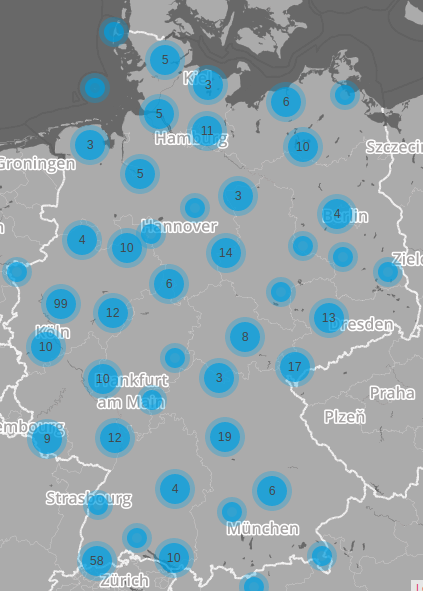
\includegraphics[width=\textwidth]{Bilder/community-map-2017-04-24}
  \end{center}
      \end{column}
    \end{columns}
  \end{frame}
  
  %-----------------
  \begin{frame}{Abmahnrisiko (früher: Störerhaftung)}
    \begin{itemize}
      \item Abmahnung auf Unterlassung denkbar
      \item Internetverkehr geht über unsere Gateways. Haftungsbefreiung nach TMG\S8.
      \item Datenschutz: Wir halten uns an die Gesetze und speichern daher nicht.
      \item Freifunk ist KEIN Anonymisierungsdienst
    \end{itemize}
  \end{frame}
  
  %-----------------
  \begin{frame}{Knotenkarte}
    \begin{center}
      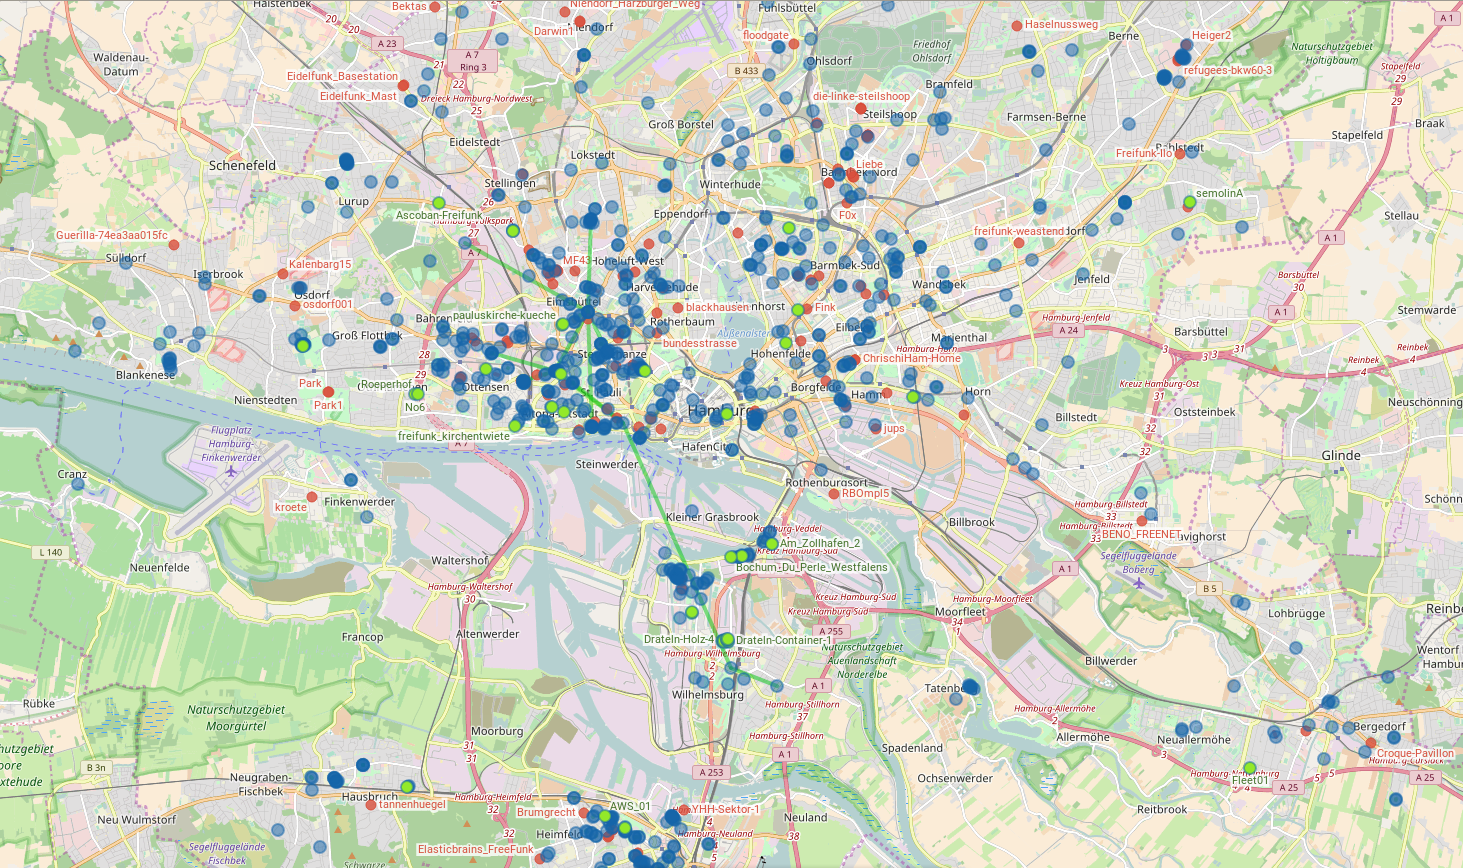
\includegraphics[width=.8\textwidth]{Bilder/knotenkarte-2017-04-24}
      \newline\tiny{Leaflet | © CC-BY-SA OpenStreetMap, andere}
    \end{center}
    Mehr als 950 Knoten in Hamburg, bis 3000 Geräte im Netz
  \end{frame}
  
  %----------------- 
  \begin{frame}{Freifunkknoten}
    \begin{center}
      \includegraphics[width=.6\textwidth]{Bilder/841}
    \end{center}
  \end{frame}
  \foreach \index in {1, ..., 4} 
  {
    \begin{frame}{Das Netzwerk}
      \centering \includesvg[width=9cm]{netz-\index}
    \end{frame}
  }
  
  %-----------------
  \begin{frame}{\href{http://wiki.freifunk.net/Hamburg/Richtfunknetz}{Richtfunknetz}}
    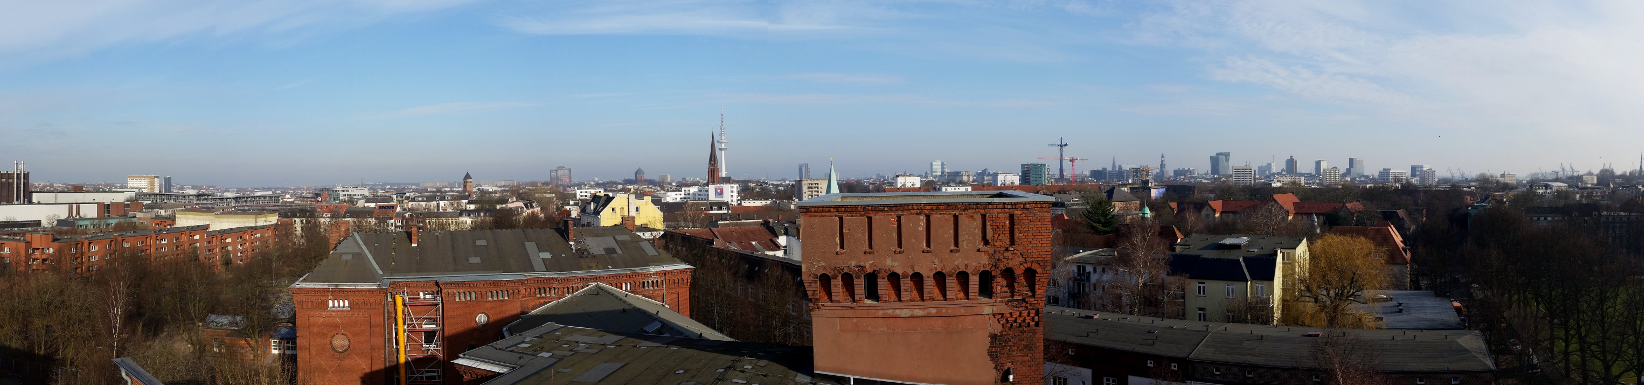
\includegraphics[width=\textwidth]{Bilder/fux-panorama}
    \begin{columns}
      \begin{column}{0.7\textwidth}
  \begin{itemize}
    \item Eigene Infrastruktur
    \begin{itemize}
      \item Redundanz und Lastverteilung 
      \item Unabhängig von Internetprovidern
    \end{itemize}
  \end{itemize}
      \end{column}
      \begin{column}{0.3\textwidth}
  \begin{center}
    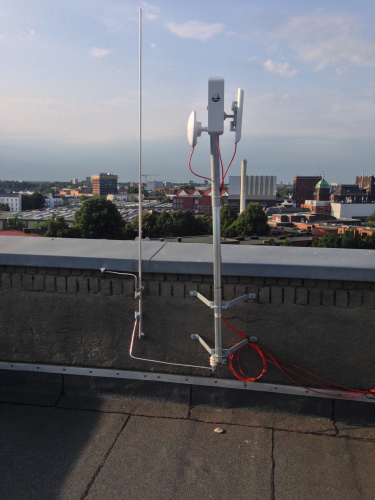
\includegraphics[width=.9\textwidth]{Bilder/richtfunkmast}
  \end{center}
      \end{column}
    \end{columns}
  \end{frame}
  
  %-----------------
  \begin{frame}{Richtfunknetz}
    \begin{center}
      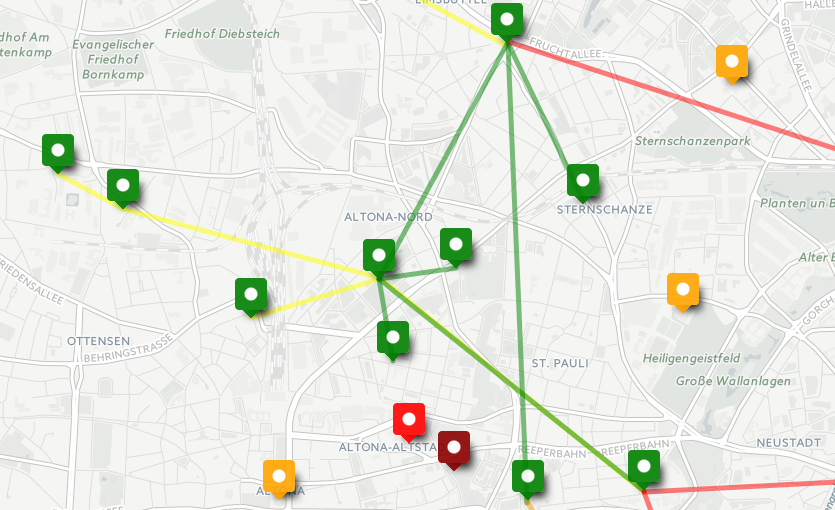
\includegraphics[width=0.95\textwidth]{Bilder/richtfunk-uebersicht}
    \end{center}
    \tiny{OSM - Deutschland Karte hergestellt aus OpenStreetMap-Daten | Lizenz: Open Database License (ODbL) | Courtesy of OpenStreetMap.de}
  \end{frame}
  
  %-----------------
  \begin{frame}{Unsere Infrastruktur}
    \begin{itemize}
      \item Unser AS: AS49009
      \item ECIX, DECIX (HH), BREM-IX, Community-IX
      \item Peerings mit anderen Freifunkern:\newline Rheinland und Berlin
      \item Peerings u.a. mit Google, Facebook, N@work, LWLcom, IPHH, Hurricane Electric
      \item > 8 TByte an Daten, jeden Tag.
    \end{itemize}
  \end{frame}
  
  %-----------------
  \begin{frame}{Flüchtlingsprojekte}
    \begin{itemize}
      \item 2013: Embassy of Hope (St. Pauli Kirche)
      \item 2014: Schwarzenbergplatz
      \item 2015 \& 2016
      \begin{itemize}
        \item Flüchtlingsschiff Transit
        \item Messehallen
        \item Hauptbahnhof
        \item mehrere alte Baumärkte
        \item ZEA Schnackenburgallee (>3000 Flüchtlinge)
        \item Zahlreiche weitere Standorte
      \end{itemize}
    \end{itemize}
  \end{frame}
  
  %-----------------
  \begin{frame}{Aktuelles\ldots}
    \begin{itemize}
      \item Vorratsdatenspeicherung
      \item Aufteilung in mehrere kleinere Netze
    \end{itemize}
  \end{frame}
  
  %-----------------
  \begin{frame}{Freifunk lebt vom Mitmachen}
    \begin{itemize}
      \item Wir sind kein Dienstleister
      \item aber wir geben unser Wissen gerne weiter
    \end{itemize}
  \end{frame}
  
  %-----------------
  \begin{frame}{Wie kann ich mitmachen?}
    \begin{itemize}
      \item Router aufstellen
      \item Freifunk Treffen
      \begin{itemize}
       \item Montags, 19 Uhr, CCCHH, Zeiseweg 9
       \item Techniktreffen Freitags, 19:30 Uhr, Attraktor, Eschelsweg 4
      \end{itemize}
      \item Website
      \begin{itemize}
       \item \href{https://hamburg.freifunk.net/}{https://hamburg.freifunk.net/}
      \end{itemize}
      \item Mailingliste
      \begin{itemize}
       \item \href{mailto:freifunk@hamburg.ccc.de}{freifunk@hamburg.ccc.de}
      \end{itemize}
      \item IRC
      \begin{itemize}
       \item \#ffhh auf irc.hackint.org
      \end{itemize}
    \end{itemize}
  \end{frame}
  
  %-----------------
  \begin{frame}{Vielen Dank!}
    \begin{center}
      \includesvg[width=3.5cm]{in-hamburg-funkt-man-frei}
    \end{center}
    \begin{itemize}
      \item Netz: \href{https://hamburg.freifunk.net}{https://hamburg.freifunk.net}
      \item Mail: \href{mailto:kontakt@hamburg.freifunk.net}{kontakt@hamburg.freifunk.net}
      \item Treffen: Montags \& Freitags, \href{https://hamburg.freifunk.net/kalender}{https://hamburg.freifunk.net/kalender}
    \end{itemize}
  \end{frame}
  
\end{document}
